\documentclass[a4paper, 11pt]{article}
%\usepackage[parfill]{parskip}
\usepackage{ragged2e}
\usepackage{graphicx}
\graphicspath{ {images/} }
%\title{Some Title I haven't decided yet}
%\author{Keimi Okamoto}
\usepackage[T1]{fontenc}

\newlength{\drop}
\usepackage{epigraph}
\usepackage{dirtytalk}
\usepackage{wrapfig}

%%%%%%%START%%%%%%%
\begin{document}
  \begin{titlepage}
    \drop=0.1\textheight
    \centering
    \vspace*{\baselineskip}
    \rule{\textwidth}{1.6pt}\vspace*{-\baselineskip}\vspace*{2pt}
    \rule{\textwidth}{0.4pt}\\[\baselineskip]
    {\Large{MSc Computer Science\\[0.3\baselineskip] }} 	
    {\huge{Project Proposal\\[0.3\baselineskip] }}
	
    \rule{\textwidth}{0.4pt}\vspace*{-\baselineskip}\vspace{3.2pt}
    \rule{\textwidth}{1.6pt}
    \\[\baselineskip]
    \scshape
    {\Large Ubiquitous Consumer Inventory Management System For Waste Prevention\\}
%    Location, date from--to\par
    \vspace*{2\baselineskip}
    %Edited by \\[\baselineskip]
    {\normalsize\emph{Supervisor: }{\large Professor George Roussos\par}}
    {\normalsize\emph{Author: }{\large Keimi Okamoto\par}}
    
    {\itshape 2015}
    \vfill
    {\large BIRKBECK UNIVERSITY OF LONDON\par}
{\footnotesize DEPARTMENT OF COMPUTER SCIENCE \& INFORMATION SYSTEMS}\par
  \end{titlepage}
  
%\maketitle
%........................
% Contents
%........................
\tableofcontents
\clearpage

%........................
% Epigraph
%........................
\centering
\setlength{\epigraphwidth}{1\textwidth\centering}
\epigraph{\say{Its highest ideal is to make a computer so exciting,
so wonderful, so interesting, that we never want to be
without it. A less-traveled path I call the \say{invisible}; its
highest ideal is to make a computer so imbedded, so fitting,
so natural, that we use it without even thinking about it. I
have also called this notion \say{Ubiquitous Computing}.}}
{\textsc{-Mark Weiser,}\textit{ `Creating the Invisible Interface' 1994}}

\clearpage
%........................
% Abstract
%........................
\abstract{Abstract}
blah blah
\clearpage

%........................
% Introduction
%........................
\section{Introduction}

\subsection{Background}
Over production of food is a global issue with waste exceeding two billion tonnes annually\cite{waste}. Such large quantities of waste has severe negative social, environmental and economical impacts. The multifaceted nature of the food supply chain give ample opportunity for waste to occur and inadequate waste prevention methods could cause figures to rise. Further more, such complex pipelines poses great difficulties in the accurate quantification of waste generated, meaning that the figures are likely to be higher than reported.\cite{waste} A clear understanding of the chain is necessary to identify the vulnerable components where waste can arise, below is a brief description of each of the three main entities that comprise the chain and their accountability to the statistics.

\paragraph{Producers}At the start exists the agriculturalists and farmers who cultivate the plants and livestocks. These entities serve as the primary source of supply to the market and respond to orders placed by retailers. Over production is often encouraged by the merchant to compensate for the possibility of an unfruitful harvest or an unexpected and sudden rise in demand.\cite{waste}

\paragraph{Retailers}The intermediator between producer and consumer are the retailers and vendors, the most dominant being Supermarkets, namely Sainsbury's, Tesco, Asda and Morrison. Perpetual competition for marketshare leads to aggressive advertising and competitive pricing wars, with millions of pounds at stake urgency for quantity control becomes a lesser priority. Errors in sales forecasts can also result to wastage or idle stock occupying valuable real-estate with rental costing millions annually. Waste can even occur on a superficial level where ascetically unpleasing but perfectly consumable food is is deemed unworthy of stocking and rejected.
%lfhw cite

\paragraph{Consumers}At the end of the chain are the consumers that are regularly persuaded to over purchase by enticing `buy-one-get-one-free' offers and other bulk buying promotions. Retailers markdown items that are nearing expiration to sell  to the consumer as an attempt to compensate for potential losses. This method of damage control while beneficial to the supermarkets have negative implications on the consumers. Loss can also occur due to basic human errors of simply forgetting to consume the food in time. Fast paced and unpredictable lifestyles attribute to the difficulties in keeping track of past purchases and expiration dates, resulting to the  contribution to the overflowing landfill sites. 

\vspace{\baselineskip}

This project will take a consumer-centric approach to tackle the issue of waste. The United Kingdom alone is estimated to generate 15 million tonnes of food waste every year, 7 million of which is accountable to domestic households.\cite{FoodWaste} Having stated this, retailers contribute largely to the figures as they strive to meet contrived demands self-orchestrated by marketing to boost revenue, causing waste that would have resided at the retailer to be pushed down the chain and ultimately dumped with the consumers. By providing consumers tools to better manage their inventory that would aid a lifestyle of maximal resource utilisation with minimum waste, demand could be controlled keeping waste at bay with the retailers. Essentially creating an upstream ripple and discouraging the over production of food by targeting the root cause of the problem.

\vspace{\baselineskip}
\vspace{\baselineskip}
\vspace{\baselineskip}

\subsection{Problem}

\begin{center}
\say{\footnotesize{\emph{It has been estimated that 89 million tonnes of food are wasted each year in the EU, a figure which could rise to approximately 126 million tonnes by 2020 if no action is taken. The United Nations' Food and Agriculture Organisation (FAO) states that every year consumers in industrialised countries waste approximately 222 million tonnes of food, which is almost as much as the entire net food production of sub-Saharan Africa, equating to 230 million tonnes.}}}\cite{FoodWaste}
\end{center}

\paragraph{Environmental}When food is wasted, this is the direct repercussion of over production and a needless contribution to the expanding carbon foot print. Processes such as pesticide application, cooking, packaging creation and disposal, distribution and temperature controlled storage all require copious amounts of fuel and energy. Waste is being generated at such a rapid rate maintaining this in landfill sites is becoming unfeasible.
%lfhw

\paragraph{Economical}A typical UK household has been reported to throw away an average of \pounds950 worth of food annually. This amounts to roughly 50kg of waste that must be collected, managed and recycled, putting pressure on councils all of which can result in higher taxes and wasted resources.\cite{FoodWaste}

\paragraph{Social} Influenced by the retailers and succumbing to the bargain deals, customers frequently over purchase food causing over consumption. Needlessly consuming to avoid loss can pose serious health risks such as obesity, diabetes, high blood pressure, and cardiovascular diseases, these are potentially life threatening and can impact the populations life expectancy and add pressure on healthcare systems. 
%houseof commons

\paragraph{Human memory}Failed stock keeping of household items is one of the primary causes of food expiring before consumption. The human brain has limited capacity to store and recall information. Research by George Armitage Miller, a prominent figure in the field of cognitive phycology discovered that the number of objects an average human can hold in working memory is seven, give or take two.\cite{memory} Foods vary in categories such as meats, fish, fruit, vegetables and nearly all come with different expiration dates, relying on memory alone is impractical. 

\paragraph{Lifestyle} Busy schedules dissuade people to use produces brought in advance and instead opt for the quick and easier choice of eating out, thus items purchased with the intentions of consumption end up as waste. Combining compatible ingredient to create an appetising dish in addition the complication of prioritising use-by-dates of fresh produces can be time consuming and an arduous task. Households usually have multiple residents and double purchasing of items is common due to break down in communication. 

\vspace{\baselineskip}
\vspace{\baselineskip}
\vspace{\baselineskip}

\subsection{Current Waste Management Methods}

\paragraph{Manual Efforts}
Various campaigns have been launched by governments across Europe with the intention to educate consumers on the implications of food waste and waste prevention methods. Such organisations as Waste \& Resources Action Programme (WRAP), a registered charity part funded by the UK Government, have been raising awareness by interacting with communities and working to promote waste avoidance. Physical interactions can be effective and inspirational but the labour force required to generate and sustain interest is costly and unmaintainable, hence the movement towards digital mediums.

\paragraph{Anaerobic Digestion}
Closed-loop solutions such as convert bio-methane gas extracted from food waste into electricity have been introduced by Sainsbury's and the waste management service Biffa. The primary goal being the powering of supermarkets with energy sourced form surplus and reducing strain on the landfill sites. The main concern for this technology is the process of converting waste to energy requires energy. 

\paragraph{Nanotechnology}
Scientists in Beijing have developed an item-level smart tag using nanotechnology to indicate when food is spoiling. The metallic nanorods in a gel mimic the length of time microbes propagate in foods. The tags alter in colour according to the presence of bacteria and each colour corresponds to the decomposition stage of the produce, thus providing visual representation of the degree of freshness. The tag react to varying tempters that can have an effect on the shelf life of a product. This technology is currently being meticulous tested to avoid any inaccuracy that could pose a potential health risk to consumers. Nanotechnology could potentially replace printed use-by-dates on products and could provide users with the an accurate reading of the longevity of food but this requires the user to manually open the fridge and memorise the colour of the tags. Presently there is no method for the tags to communicate.

\paragraph{Mobile Applications}
With most people owning Smartphones and as a result of Apple and Google's infamous App Stores, the instantaneous time to market is hugely advantageous to businesses and organisations. 

`Love Food, Hate Waste' (LFHW), a campaign launched by WRAP, which primarily operates through an interactive website have developed an app with helpful features such as a shopping lists memo maker, recipe suggestions, portion size suggestions. Other governments are also promoting the use of mobile applications. `Smart Cooking' developed by the Netherlands Nutrition Centre Foundation (NNCF) funded by the Dutch government incorporates similar features to LFHW. TooSkee and LeanPath are other examples of food management apps. Developed in the US, receipts are scanned and items are logged. Much like the other mobile applications it will suggest dishes and remind the user to consume products before the expiration date. Dates must be entered manually as barcodes are not able to provide this information. 

Without question Smartphone apps are the most effective way to deliver the software to the consumer but with an over-crowded market place where a single bad review can jeopardise the success of an app, quality and functionality is paramount as users have become increasingly intolerant of a poor interface design or performance such as delayed content loading.

\paragraph{SmartFridge}
This internet enabled appliance was designed for home food management including the automated replenishment of stock. The user will scan products using a laser built into the fridge and recipes are suggested depending on the content. Inventory information is accessible through a Smart device either provided by the manufacture or via Smartphone. This eagerly anticipated technological innovation was somewhat anti-climatic as flaws in the practicality of the product surfaced. Items had to be manually entered due to the lack data and the recommendations were not as helpful as initially thought, together with the unit costing over \$20,000 many were reluctant to invest.

\paragraph{Radio Frequency Identification (RFID)}
Dutch researchers form NXP Semiconductors have collaborated with the Netherlands Packaging Centre (NPC),  to develop a sensor enabled RFID tag capable of monitoring environmental changes food is exposed to through the supply chain. The Pasteur sensor tag has the capacity of measuring shifts in temperature and gas conditions during transportation and various stages of storage. This data is analysed to give an accurate reading of the products shelf life, thus being able to prioritise the trading of supplies and reducing the likelihood of waste. At the currents state this is only available at the producer-level for the shipment of large volumes to suppliers. 

The use of RFID has been prevalent in the supply chain but it is yet to be deployed at the item-level and is primarily used for asset monitoring rather than waste management. RFID in the supply chain has gained recognition for it's contribution to real-time stock monitoring and the simplistic way in which shipments can be identified. The next section will discuss the current method of identification at the item-level and how RFID can offer transparency and efficiency, much like it has at the producer and supplier level.


\vspace{\baselineskip}
\vspace{\baselineskip}
\vspace{\baselineskip}

\subsection{Product Identification}

\subsubsection{RFID vs Barcodes}Currently barcodes are the most widely used method of item identification. Barcodes have been implemented in the supply chain since the 1970's for stock monitoring and sales total analysis as well as the acceleration and digitalisation of the checkout process. Barcode are universally recognised, inexpensive to print and many businesses have the printing process built into the production line, making it difficult for manufacturers accept other technologies. However, there are a few disadvantages to this technology. Firstly, for the barcode to be read successfully there must be no obstructions between the laser and the barcode, this includes dirt or scratches that distort the image. Secondly, the laser must be kept parallel to the barcode for a successful read and simultaneous scanning is not possible. It is also note worthy to mention that barcodes are unique to the product type but not at the item-level. For example it is not possible to distinguish the difference between one carton of milk and another made by the same manufacturer, meaning a machine is not able to distinguish one item from another.

In contrast, RFID does not require a laser as it utilises electromagnetic radio fields for communication. So long as the tag is within the vicinity of the field it can be read and even facilitate the simultaneous reads of multiple tags. Tag have varied memory capacity but typically very low usually the size of a URL can be stored, this is enough to bridge between object and the internet where additional data can be stored or updated as external data storage is abundantly available. Uniform Resource Locator's (URL) also provide individuality to an object, allowing customised granular information to be stored and accessible. Once the barcode is printed it is hardcoded on to the product giving little room for errors but with RFID remote alterations of the product is possible.

RFID offerers simplicity as demonstrated by contactless payment and the Oyster card for the London transport system. RFID is also already prevalent in supply chains to monitor and track stock and even livestock. Companies such Marks \& Spenser have tagged their clothing for inventory keeping and theft prevention. As the popularity rises some will question whether item-level uniqueness is a necessity for the food supply chain, where the product lifecycle can be as short as a few days and if the practical values out weigh the economical penalties. 

\vspace{\baselineskip}
\vspace{\baselineskip}
\vspace{\baselineskip}

\subsubsection{Importance of Item-Level Identification}

\paragraph{Remote Amendment of Human Errors}
Perfectly consumable foods is regularly recalled and wasted due to human errors such as misprinted information on the label or neglecting to provide information that abide by food standard regulations. With RFID tags can be updated remotely issuing immediate alerts to consumers of the mistake and the amended error. This provides a different approach to error management.

\paragraph{Food Safety and traceability}
In the past there has been numerous incidents when products have been recalled due to the presence of bacteria or other abnormalities. A notable incident is the 2013 meat adulteration scandal in the EU, where traces of horse meat where discovered in various products such as minced meat and ready prepared meals. The time and resources to trace back through the supply chain was estimated to have cost the Food Standard Agency (FSA) \pounds900,000 between 2011 and 2012 and a further \pounds1.6 million between 2012 and 2013 \cite{3}. Other casualties include the reputations and integrity of the blameless producers falsely accused due to inaccurate data that implicated them as the guilty.\cite{horse}

With item-level identification the contaminated produce could be traced back immediately and the products recalled. For example if an infected animal is used in various products, all items holding that particular code can be instantly traceable, compartmentalising the outbreak and maximising efficiency in damage control. 

\paragraph{Transparency \& Consumer Rights}
The law enforces that labels of fresh meat must contain the country of origin, but this does not apply to the same meat that are processed, such as hamburgers, pies and sausages. (cite article 18) Meats may also be mixed providing that the animals are slaughtered in the same country, meaning a single hamburger could be made up of several cows. 

The Regulations of the EU parliament and council state that abattoirs and agriculturalists must provide documentation containing country of birth, rearing, slaughter, cutting along with slaughterhouse and cutting plant approval numbers for the product(cite) when sourcing retailers or informing officials. But this is not enforced at the consumer level, meaning the information is not being passed down. It is evident that meats in particular have unique backgrounds. Ranging from the rearing environments, type of feed consumed and drugs administered. This information can help make consumers make better decisions whether it is for health reasons, environmental or ethically conscious individuals. The Food Standard Agency published a report on the labelling guidance of food:

\vspace{\baselineskip}
\say{\emph{It is clear that many consumers want more information on the origin of meat ingredients in meat products, and in the Agency's consumer research the ingredients in dairy produce also score highly in this respect. The law requires an origin declaration on fresh beef but not on the same product when it has been seasoned. Providing information on the origin of all ingredients in all products would be disproportionately burdensome for industry, and would risk overloading the label with information that is not
seen as important by consumers.}} {\textsc{- Food Standard Agency}\textit{`country of origin labelling guidence'}
\vspace{\baselineskip}

With the use of RFID the overloading of the label would no longer be a reason to with hold information from the consumer and the consumers as individuals can decide what information is of importance.

Such areas as Japan where vegetables and livestock were exposed to nuclear radiation due to the Fukushima Daiichi nuclear disaster raises serious health concerns for the consumer. Damage caused by radiation exposure by consumption of contaminated foods can surface much later in a persons life\cite{fukushima} and in some cases even be inherited by offspring. This highlights the urgency for transpicuous detail of the product's life cycle and the importance for the consumer to be fully aware of the risks and responsible for what they choose to consume.

\paragraph{Personal Recommendation} As well as waste management item-level identification can benefit other areas of the supply chain. Personalised promotions and predictive suggestions can increase productivity for the consumer and shopping experience can be greatly enhanced as demonstrated by MyGROCER\cite{myGrocer}. A system that integrated RFID into a supermarket to fully automate the check out process. MyGROCER provided the consumer with a shopping cart embedded with readers that were able to log the items and transmit the total purchases to the cashier, removing the time consuming task of item scanning. This system proved that the enablement of RFID technology in the supply chain and the creating of ubiquitous objects was beneficial to both consumer and supplier. The concept of objects capable of acknowledging the presence of another objects exhibits the efficiency ubiquitous computing can provide.

\vspace{\baselineskip}
\vspace{\baselineskip}
\vspace{\baselineskip}

\subsection{Ubiquitous Computing}

\paragraph{Brief history} Mark Weiser who has been credited as the founding father of the movement as well as the coining of the paradigm was motivated by the notion that any person may access any information in any place at any time.\cite{weiser} This notion of peer aware devices generating a response composed of shared logic for the betterment of our lives continues to influence the development of smart devices and internet enabled objects today.  

One of the first appliance to be placed online was a Coca-Cola vending machine developed in Carnegie Mellon University in 1982. Users were able to connect via the internet and check whether the canned beverages were chilled. This information would be the deciding factor on whether the user would make the trip to the machine. This technological breakthrough gave an insight into a new era were objects were able to cater to our immediate needs. With the enablement of machine to machine communications, a once passive and inanimate object is able to actively communicate with other `things' through a network, sharing data and working harmoniously to maximise efficiency to permissively aid our everyday lives.

\paragraph{RFID \& Cloud Services}One of the fundamental bottlenecks to Weiser's research was the limitations of computational power available in 1993\cite{weiserLimit}, together with inability for hardware advancements to catch up with his vision. Over ten years on, computers have become increasingly compact and portable that the need for desktop machines are decreasing. Cloud vendors such as Amazon and Google offer huge computational power utilising comodity hardware in the form of Cloud Services that Moore's law is no longer applicable\cite{HadoopInAction}. 

As the popularity in RFID technology rises and increasing amounts of physical object become internet enabled the need for parallel high-speed computing becomes evident. The dynamic provisioning of shared pooled resources makes for a highly scalable infrastructure that is favourable to ubiquitous systems which potentially process large quantities of user generated content. Peaks and troughs of demand fluctuation are automatically managed and massive amounts of data can be computed in parallel in a matter of seconds. This is highly desirable for the food supply chain where large quantities of produce is churned out daily. Cloud services also support the interoperable aspect of ubiquitous systems, Amazon Web Services and Google App Engine both provide highly compatible and uniform API's that can be `plugged and played' by devices varying in operating systems flavours and hardware giving room for expansion and flexibility. Many vendors also have elegant and autonomous fault detection protocols that are able to self-healing with minimal, if not, the complete elimination of human intervention. Cloud services also bring economical merits with a `pay-for-what-you-use' utility based billing method and is in favour of green computing. With GS1's efforts to standardise the identification methods of products using RFID with electronic product codes, a unique identifier, and the movement towards providing a unique identification for every physical object in the world highlights the need for high-speed computational capabilities and accessibility. 

\paragraph{Smartphones}Smartphones have undoubtably accelerated the movement of ubiquitous computing and have earned a monumental position in the everyday lives of people. With many Smartphones equipped with multiple sensors including RFID, external devices are able to transmit and receive information to and from it's owner with ease. This practicality lends it's self to being the most successful smart device on the market. app-stores are able to deliver software quite literally into the palms of the users hands shortening the gap of traditional development to market delivery time. 

\clearpage

%........................
% Aims & Objectives
%........................
\section{Aims and Objectives}
\subsection{Aims}

The aim is to demonstrate the use of item-level RFID tagging of food products to support the positive contribution to waste reduction. The system should seamlessly integrate into the domestic home environment and aid the consumer with personal inventory management and assisting in the optimum utilisation of resources for the inhabitants. 

As mentioned previously, content monitoring apps are readily available to consumers. But after analysis of the technologies such as the Smart Fridge and the LFHW waste management App, it became evident that the arduous steps necessary to register the items rendered it incompatible with the hectic modern lifestyle of the consumers. Items must be scanned item by item with careful precision, lining up the laser and barcode for a successful reads. If there are any obstructions the item will be inaccessible and manual intervention is required. Even after a successful read the information accessible digitally is limited and crucial details such as use-by-dates requires manual input from the user. This shortcoming of the process hinders the usability of such technologies and with finite memory on smartphones, real-estate is valuable and Apps are discarded and forgotten just as quickly as they were installed.

\begin{figure}[h!]
  \centering
    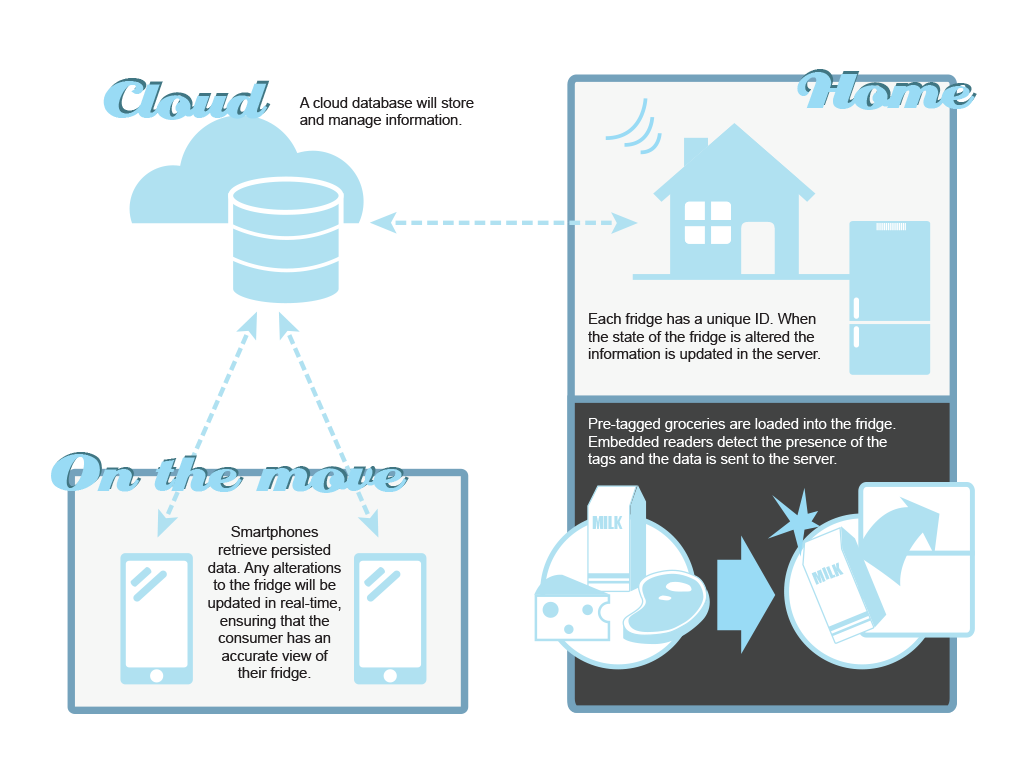
\includegraphics[width=0.9\textwidth]{system2.png}
      \caption{demo}
\end{figure}

\paragraph{Concept}The proposed concept will incorporate RFID technology as a means of registration. Items will be pre-tagged and granular item-level detail such as use-by-dates and ingredients accessible. There will be no need to alter the consumers usual behaviour and process of restocking their fridge. Items simply need to be placed in the fridge as usual and the readers will recognise the items automatically. As the fridge door closes readers will scan the fridge and record any changes keeping the inventory up to date. Data can be stored using a cloud database giving plenty of leeway for future expansion and highly scalable data retrieval and persistence mechanisms. The information captured will be organised, analysed and presented to the consumer in an user-friendly format via a Smartphone. By equipping the consumer with an app, waste can be reduced and over purchasing can be avoided. The following points will provide solutions and articulate how the app intends to overcome the current issues stated in part one.

\vspace{\baselineskip}

\begin{itemize}
  \item Instant look-up of the content of the fridge when away from the home. This feature is intended to dissuade excessive purchasing of groceries and to support the consumer to make a better judgements when faced with detrimental promotional offers from supermarkets.
  
  \item Real-time state monitoring and logging of items. In a scenario where the home has multiple inhabitants the state of the fridge can be altered without all members being aware, the system will keep all inhabitants informed when items are added or removed, avoiding duplicate purchasing and monetary waste.
  
  \item Tracking and prioritisation of foods that need to be consumed in accordance to the use-by-date eliminating the need for consumers to memorise to use certain products. 
  
  \item Statistics analysis of the amount of money they have thrown away can provide motivation for the user to consume purchased foods and encourage them to minimise wastage.
   
   \item Automated meal planning feature using the contents of the fridge alleviating the time consuming process of co-ordinating meals. 
    
   \item Helpful hints such as cooking and freezing to extend the longevity of food. 
   
   \item Recommendation for recipes depending on current inventory to inspire the consumer to create suggested dishes. 

   \item Optimal stocking advice relative to the number of inhabitants and shopping list generation depending on previous purchases. 
 \end{itemize}

To further clarify the functionality of the App the given hypothetical scenario will evoke a vision of how the app will aid the domestic environment. 

\paragraph{Scenario}On the way home from work Rachel visits the supermarket. She consults her smartphone for a reminder of what her fridge contains back at home. A shopping list has been generated for her. She will need less food than the previous week as she has a family dinner scheduled at her mother's this weekend. She browses the poultry aisle and notices a special offer on chicken, `Buy two get the third free' the label reads. According to the application the fridge already contains chicken that must be consumed by tomorrow. She decides against the purchase and carries on, the next item on the list is milk. But then her phone notifies her that her husband Frank has just stocked the fridge with a one litre carton of semi-skimmed milk. She completes the shopping and arrives home and restocks the fridge. Her daughter Ingrid is on the way home from college, her parents are working late and she must prepare dinner for herself and younger brother Dean this evening. As she scrolls through the items on the screen of the smartPhone the app recommends cheese and onion quiche, ready in 20 minutes and one of Dean's favourites. After dinner Ingrid decides to prepare desert, as she unloads the cheesecake from the fridge her Smartphone signals a warning that the cheesecake contains gelatine. Ingrid is a vegetarian, she opts for the yoghurt instead and serves the cheesecake to her brother. At the end of the week a visual chart representing the analysis of the families savings and quantity of food consumed is broadcasted to all members.

\paragraph{Further Extension\dots} This concept can be expanded to other storage locations such as the pantry or freezer. As more objects become live and the network expands, systems become increasingly sophisticated sharing data to evolve. Popular wearable devices such as fitness trackers that calculate the amount of calories exhausted can work cooperatively with the home inventory management system and recommend the optimal diet for the individual to lead a healthy lifestyle. Smart shopping solutions such as MyGROCER\cite{myGrocer} will be able to work with the smart fridge and responsibly source personalised promotions sent directly to the consumer.

\vspace{\baselineskip}
\vspace{\baselineskip}
\vspace{\baselineskip}

\subsection{Limitations}

\paragraph{Infrastructure}Although the technology is available the primary set back is the lack of infrastructure in place to support RFID enabled grocery products. It would require significant changes to the supply chain and business processes \cite{pervasiveComp} as experienced by MyGROCER. Barcode printing has it's roots firmly planted in the supply chain and the transition to RFID labelling is slow. With this restriction the prototype will be setup in a hypothetical environment.

\paragraph{Cost and Environment}Food is mass produced daily resulting in large scale utilisation of tags, this raises concerns for the environment as tags contain non-biodegradable materials such as metal, plastic and petrochemical based materials.\cite{bioTags} Research and production of biodegradable RFID tags are progressing but at the present time it is not available. In the past cost has also effected the move to RFID usage for groceries. The cost of tags has significantly decreased over the past decade but including the process of tagging in the supply chain work flow would still require new machinery and alteration to current operations. 

\paragraph{Privacy}Data persistence is a fundamental part of most systems. As systems advance the concerns over privacy become a controversial topic. At some point, for some length, data must be stored giving opportunities for unethical practice that can lead to the abuse and exploitations of an individual. This seems to be a double edged sword as when data is used in a responsible and respectful manner it is able to provide us with great advancements to our lives but on the other side, ramification of bad practices can be disruptive and invasive.
\clearpage

\subsection{Objectives}
The objectives have been stated with consideration given to the time allocated to complete the project. The primary deliverable will take the form of a simple proof of concept to be further developed at a later date. 

\begin{enumerate}

   \item \textbf{Obtain Knowledge of RFID classifications and Reader capabilities}
   	\begin{flushleft}Investigating various classifications of RFID tags and readers to better understand the capabilities and limitation. Based on acquired knowledge, one should achieve the expertise to critically assess and select the most appropriate hardware for the use-case of the project.
  	\end{flushleft}
	
   \item \textbf{Tag and Reader Prototype Setup}
   	\begin{flushleft}Gaining the understanding of the technological underpinnings of RFID technology and tag to reader communications. Successful hardware configuration for demonstration purposes.
  	\end{flushleft}
  
   \item \textbf{Front End Development}
   	\begin{flushleft}Front end development of a simple graphical user interface with minimal functionality, using the Android software development kit (SDK) that will engage with the user. User will view an itemised list of their current inventory.
		  \end{flushleft}
  
   \item \textbf{Back End Configuration of Third-Party Cloud Service}
   	\begin{flushleft}
	Backend configuration using cloud service and exploring cloud service API's.  Gaining experience of using third-party softwares and API's and methods of integration. Managing responses from the client side. 
	 \end{flushleft}
	 
	    \item \textbf{Front end, back end Integration}
   	\begin{flushleft}Understanding the RFID stack and how different components are architected. Managing compatibility issues and adapting to potential change.
  	\end{flushleft}
 
  \item \textbf{Testing}
   	\begin{flushleft}Delivery of maintainable and transferable code. Gaining confidence and understanding of best practices for production code development. Manual testing using a simple graphical user interface to support the demonstration.
 	\end{flushleft}
 
 \item \textbf{Product Demonstration}
 	\begin{flushleft}A short demonstration and critical evaluation of the prototype. Discussion of the functionality of the application and discoveries and constraints encountered.
 	\end{flushleft}
\end{enumerate}
\clearpage


%........................
% Methodology
%........................
\section{Methodology}

\subsection{System Overview \& Communication Paths}

The front end of the system will 
To better understand the development proccess Figure 2 depicts the system overview and levels in which the components sit. Directed communication paths  

  \vspace{\baselineskip}
\begin{figure}[h!]
  \centering
    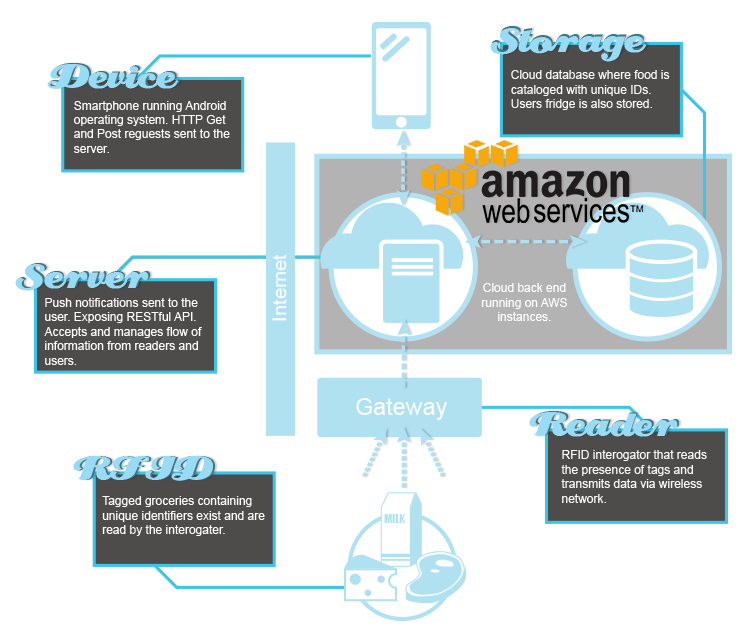
\includegraphics[width=0.9\textwidth]{system6.png}
      \caption{High-Level System Overview.}
\end{figure}

\subsection{Development}
Below are stages of development with primary deliverables in correspondence to the objectives in the previous section.

\begin{enumerate}
%1
   \item \textbf{Select RFID \& Label Groceries}
   	\begin{flushleft}Firstly, research on currently available RFID tags will be carried out to understand the limitations and capabilities that will influence the final choice. Cost, range and compatibility will be taken into consideration when selecting a appropriate tag for the use-case. Secondly, investigation of existing systems using RFID to further understand the technology. 
	
	\emph{\textbf{Outcome:}} Selection and application of appropriate tags, together will explanation and backup of the decision, followed by discuss potential pay-offs that may have influenced the final choice.
	  	\end{flushleft}
	  \vspace{\baselineskip}
	  \vspace{\baselineskip}
   \item \textbf{Research RFID stack}
%2
   	\begin{flushleft}Research the RFID stack and the nessasry componets to support introperbility and understanding the functionality of the layers that comprise the stack. Knowledge obtained may highlight potential risks and difficulties that lie ahead.
	
	\emph{\textbf{Outcome:}}Awareness of the various layers of the stack. System design and architecture established. \end{flushleft}
	  \vspace{\baselineskip}
%3
   \item \textbf{Setting up the development environment}
   	\begin{flushleft}Installation of integrated development environment(IDE), software development kit,(SDK), importing libraries and plugins. RFID enabled Android phone will be used as the reader and a testing platform.  
		
		\emph{\textbf{Outcome:}}  Setup of an environment fit to begin development.
		\end{flushleft}
	  \vspace{\baselineskip}
%4
	   \item \textbf{Front end development with Android}
   	\begin{flushleft}Using Android SDK develop a client application to manage reader to tag communications. Java will be the chosen language as supported by the SDK.
	
	\emph{\textbf{Outcome:}} A java interface using the RESTful API. Implementation and development of client to send requests to sever. Simple Graphical user interface will little functionality to trigger requests. 	
	\end{flushleft}
	\vspace{\baselineskip}
 
%5
   \item \textbf{Back end Configuration }
   	\begin{flushleft}Backend development using AWS' mobile development SDK. Using Amazon's Lambda API, client messages will be managed. Main logic of the application developed.
	
	\emph{\textbf{Outcome:}} Main logic implemented. Program that logs the contents of the fridge and updates the client when the state of the fridge is altered. Priority listing of items that the consumer can view through Android device. Successful Messages and request handeling form server.
	\vspace{\baselineskip}
  	\end{flushleft}
%6	
	   \item \textbf{Cloud Database Integration}
   	\begin{flushleft} Configure Amazons DynamoDB to respond to server requests. Create a central database for global product information to be stored. Fridge identifier and inventory to also be stored.
	
	\emph{\textbf{Outcome:}} Data persisted and server is able to respond to 
	\vspace{\baselineskip}
  	\end{flushleft}
	  \vspace{\baselineskip}
	  
%7	
   \item \textbf{Testing}
   	\begin{flushleft}Testing of the application will be carried out and documented throughout the process. Reflection of test results and assessment of the next process will be carried out. 
  	
	\emph{\textbf{Outcome:}} Documentation of test results and critical analysis of each stage. 
	\vspace{\baselineskip}
  	\end{flushleft}
%8	
	   \item \textbf{Demonstration}
   	\begin{flushleft}Demonstrate the functionality of the prototype.
	
	\emph{\textbf{Outcome:}}A proof of concept in the form of an Android application with simple functionality.

  	\end{flushleft}
\end{enumerate}
\vspace{\baselineskip}

\paragraph{Agile}With the heavy use of new and complex technologies the favourable approach is the agile development methodology. Incremental sprints offers flexibility and quick and dirty prototypes are outputted for fast feedback. This proccess responds well to change and unpredictable development processes. With the project being an idivisule effort the project will not be able to follow a pure form of agile but will At the start of each day objectives and targets will be established for each sprint deliverables will be stated in responce to previous sprints and nessary changes made.

\vspace{\baselineskip}
\vspace{\baselineskip}
\vspace{\baselineskip}

\subsection{Risks \& Pitfalls}
\paragraph{New Technology}With the use of new technology there is a high possibility of unforseen problems to arise. Solving the issue could slow the development process. Originally planned and organised decisions may be forced to change. Responding to change and managing enhancement to pay-off balancing could be tough. 

\paragraph{Compatibility \& Languages}As with most complex and new systems compatibility of components could cause production. 
\clearpage

%........................
% Schedule
%........................
\section{Schedule}
\subsection{Timetable}

\paragraph{\textbf{Week 1: 8th June:	}} Hi

\paragraph{\textbf{Week 1: 8th June:	}} 

\paragraph{\textbf{Week 1: 8th June:	}} 


Reseach of RFID	

Week 2


13 weeks
14 September 2015- DEADLINE

\clearpage
%........................
% Bibliography
%........................


% [5] U. J. Gelinas, et al., Business Processes and Information Technology. Cincinnati: South-Western/%Thomson Learning, 2004.
\begin{thebibliography}{15}

\bibitem{waste}W. Carr, E.Downing, \emph{Food Waste}, Science and Environment Section, House of Commons, 2 December 2014
\vspace{\baselineskip}

\bibitem{FoodWaste}European Union Committee, \emph{Counting the Cost of Food Waste: EU Food Waste Prevention}, London : The Stationery Office Limited, House of Lords, 6 April 2014
\vspace{\baselineskip}

\bibitem{memory}G.A Miller, \emph{Magical Number Seven, Plus or Minus Two: Some Limits on Our Capacity for Processing Information}, vol. 63. Cambridge, MA: The Psychological Review, 1956.
\vspace{\baselineskip}

%add horsy
\bibitem{horse}
\vspace{\baselineskip}

\bibitem{3}
Environment, Food and Rural Affairs Committee: Evidence,
example:Article 3 of Commission Implementing Regulation EU
\vspace{\baselineskip}

\bibitem{fukushima}World Health Organisation, \emph{Health risk assessment from the nuclear accidentafter the 2011 Great East Japan Earthquake and Tsunami based on a preliminary dose estimation}, ISBN9789241505130 Geneva, Switzerland: WHO Press, 2013
\vspace{\baselineskip}

\bibitem{myGrocer}Panos Kourouthanasis, Diomidis Spinellis, Giorgos Roussos, and Giorgos Giaglis, \emph{Intelligent Cokes and Diapers: MyGROCER Ubiquitous Computing Environment}, First International Mobile Business Conference, July 2002
\vspace{\baselineskip}

\bibitem{weiserLimit}M. Weiser, \emph{Some Computer Science Issues in Ubiquitous Computing}, CACM, July 1993
\vspace{\baselineskip}

\bibitem{HadoopInAction}C. Lam, \emph{Hadoop in Action}, 1st edition, Manning Publications, 25th Dec. 2010
\vspace{\baselineskip}

\bibitem{pervasiveComp}

\bibitem{bioTags}Y. Duroc, D. Kaddour, \emph{RFID potential impacts and future evolution for green projects},26000 Valence, France, Elsevier Ltd, 2012
\end{thebibliography}
\end{document}
%%%
\setlength{\parindent}{0pt}
\begin{document}


\end{document}
